\begin{titlepage}

\newcommand{\HRule}{\rule{\linewidth}{0.5mm}} % Defines a new command for the horizontal lines, change thickness here

\center % Center everything on the page 
%----------------------------------------------------------------------------------------
%	HEADING 
%----------------------------------------------------------------------------------------
\textsc{\LARGE École Polytechnique Fédérale de Lausanne}\\[1.5cm] % Name of your university/college
\textsc{\Large Méthodes de Production}\\[0.5cm] % Major heading such as course name

%----------------------------------------------------------------------------------------
%	TITLE 
%----------------------------------------------------------------------------------------
\HRule \\[0.4cm]
{ \huge \bfseries Molded Interconnect Devices}\\[0.4cm] % Title of your document
\HRule \\[1.5cm]
 
%----------------------------------------------------------------------------------------
% LOGO EPFL
%----------------------------------------------------------------------------------------
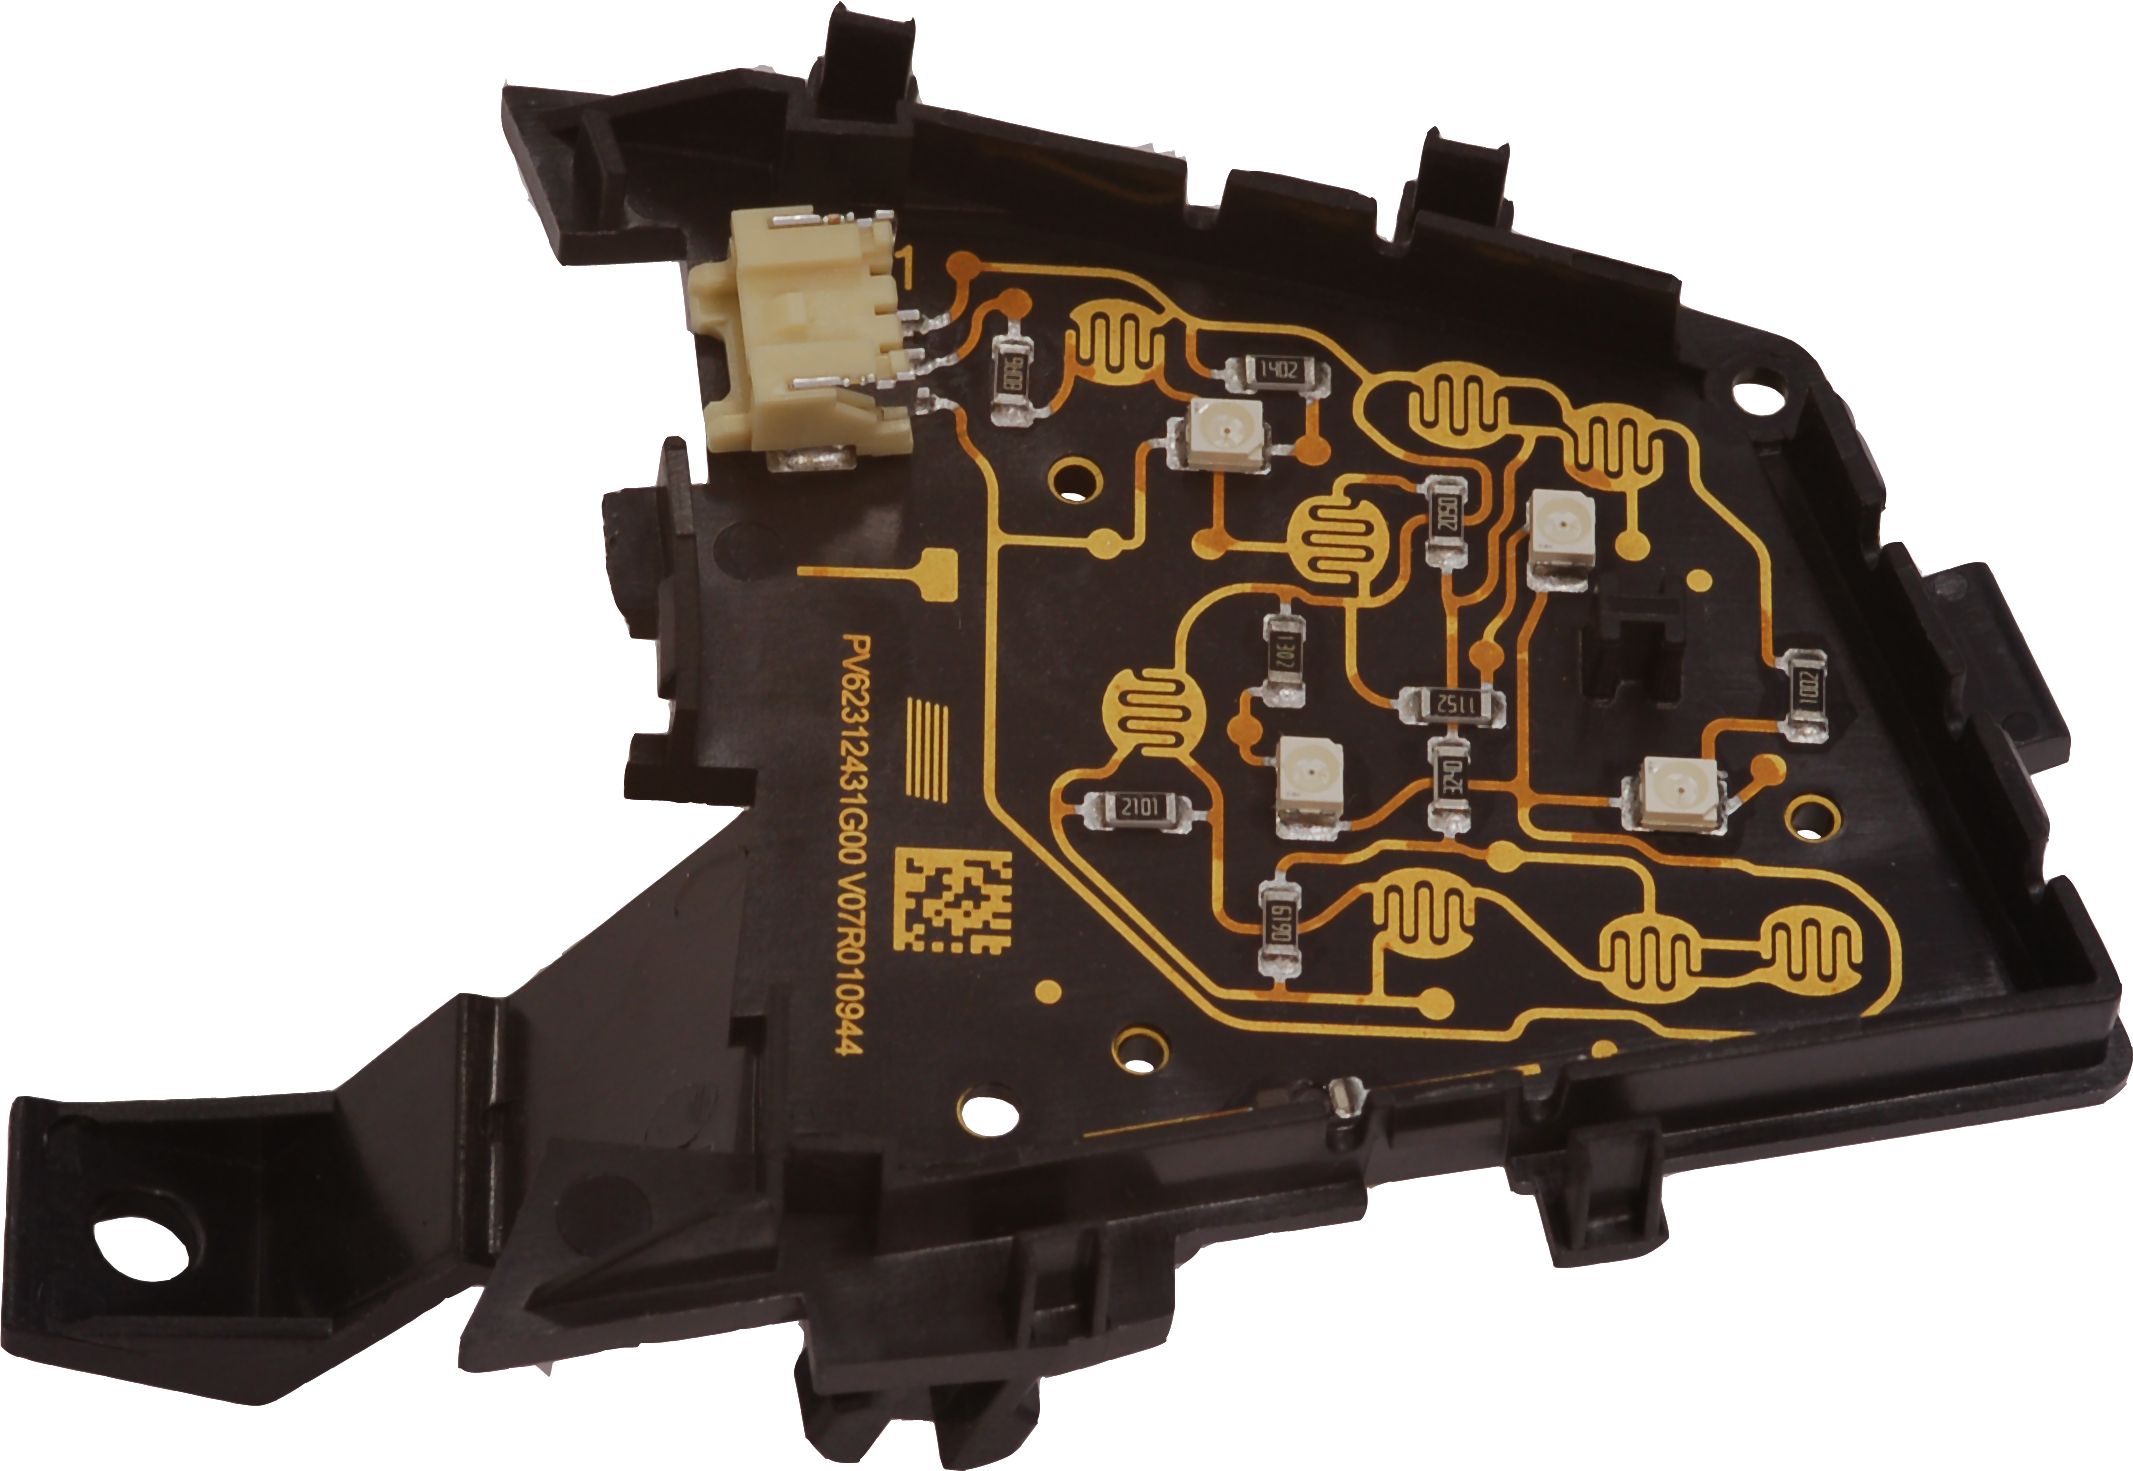
\includegraphics[width=0.8\textwidth]{mid_example}\\[3cm] 

%----------------------------------------------------------------------------------------
%	AUTHORS 
%----------------------------------------------------------------------------------------

\vfill % Fill the rest of the page with whitespace
\begin{minipage}{0.4\textwidth}
\begin{flushleft} \large
\emph{Étudiants:}\\
Antoine \textsc{Albertelli} 
Quentin \textsc{Herzig}
\end{flushleft}
\end{minipage}
~
\begin{minipage}{0.4\textwidth}
\begin{flushright} \large
\emph{Enseignants:} \\
Pr. Jacques \textsc{Jacot} \\
Dr. Jean-Daniel \textsc{Lüthi}
\end{flushright}
\end{minipage}\\[2cm]


{\large \today}
\end{titlepage}


